\documentclass{bmcart}

\usepackage{amsthm,amsmath}
\usepackage{dsfont}
\usepackage[utf8]{inputenc}
\usepackage{url}
\usepackage{color}
\usepackage{xspace}
\usepackage{graphicx}
\usepackage{hyperref}
\usepackage{relsize}
\usepackage{siunitx}
% \def\includegraphic[#1]{}
% \def\includegraphics[#1]{}

\newcommand{\lnameref}[1]{%
\bgroup
\let\nmu\MakeLowercase
\nameref{#1}\egroup}
\newcommand{\fnameref}[1]{%
\bgroup
\def\nmu{\let\nmu\MakeLowercase}%
\nameref{#1}\egroup}

\newcommand{\nmu}{}

%%% Put your definitions there:
\startlocaldefs

\newcommand*{\eg}{e.g.,\@\xspace}
\newcommand*{\ie}{i.e.,\@\xspace}
\newcommand*{\vs}{vs.\@\xspace}

\newcommand{\ipt}{IPT\xspace}
\newcommand{\ipts}{IPTs\xspace}

\newcommand{\patk}{p\mathrm{@}k}

\newcommand{\Card}{\mathrm{card}}

\newcommand{\ml}[1]{\textcolor{blue}{ML: #1}\xspace}
\newcommand{\vl}[1]{\textcolor{red}{VL: #1}\xspace}
\newcommand{\ja}[1]{\textcolor{purple}{JA: #1}\xspace}

\endlocaldefs


%%% Begin ...
\begin{document}

%%% Start of article front matter
\begin{frontmatter}

\begin{fmbox}
\dochead{Research}

%%%%%%%%%%%%%%%%%%%%%%%%%%%%%%%%%%%%%%%%%%%%%%
%%                                          %%
%% Enter the title of your article here     %%
%%                                          %%
%%%%%%%%%%%%%%%%%%%%%%%%%%%%%%%%%%%%%%%%%%%%%%

\title{Learning Auditory Similarities Between Instrumental Playing Techniques}

%%%%%%%%%%%%%%%%%%%%%%%%%%%%%%%%%%%%%%%%%%%%%%
%%                                          %%
%% Enter the authors here                   %%
%%                                          %%
%% Specify information, if available,       %%
%% in the form:                             %%
%%   <key>={<id1>,<id2>}                    %%
%%   <key>=                                 %%
%% Comment or delete the keys which are     %%
%% not used. Repeat \author command as much %%
%% as required.                             %%
%%                                          %%
%%%%%%%%%%%%%%%%%%%%%%%%%%%%%%%%%%%%%%%%%%%%%%

\author[
   addressref={aff1},                   % id's of addresses, e.g. {aff1,aff2}
                        % id of corresponding address, if any
%   noteref={n1},                        % id's of article notes, if any
   email={vincent.lostanlen@nyu.edu}            % email address
]{\inits{VL}\fnm{Vincent} \snm{Lostanlen}}
\author[
   addressref={aff2},
   email={christian.elhajj@ls2n.fr}
]{\inits{CE}\fnm{Christian} \snm{El-Hajj}}
\author[
   addressref={aff3},
   email={mathias.rossignol@lonofi.com}
]{\inits{MR}\fnm{Mathias} \snm{Rossignol}}
\author[
   addressref={aff3},
   email={gregoire.lafay@lonofi.com}
]{\inits{GL}\fnm{Gr\'egoire} \snm{Lafay}}
\author[
   addressref={ccm},
   email={janden@flatironinstitute.org}
]{\inits{JA}\fnm{Joakim} \snm{And\'en}}
\author[
  corref={aff2},
  addressref={aff2},
  email={mathieu.lagrange@ls2n.fr}
]{\inits{ML}\fnm{Mathieu} \snm{Lagrange}}

%%%%%%%%%%%%%%%%%%%%%%%%%%%%%%%%%%%%%%%%%%%%%%
%%                                          %%
%% Enter the authors' addresses here        %%
%%                                          %%
%% Repeat \address commands as much as      %%
%% required.                                %%
%%                                          %%
%%%%%%%%%%%%%%%%%%%%%%%%%%%%%%%%%%%%%%%%%%%%%%

\address[id=aff1]{%                           % unique id
  \orgname{Music and Audio Research Lab, New York University}, % university, etc
  \street{370 Jay Street},                     %
  %\postcode{}                                % post or zip code
  \city{New York, NY},                              % city
  \cny{USA}                                    % country
}
\address[id=aff2]{%
  \orgname{LS2N, CNRS, Centrale Nantes, Nantes University},
  \street{1, rue de la Noe},
  \postcode{44000},
  \city{Nantes},
  \cny{France}
}
\address[id=aff3]{%
  \orgname{Lonofi},
  \street{57 rue Letort},
  \postcode{75018},
  \city{Paris},
  \cny{France}
}
\address[id=ccm]{%
  \orgname{Center for Computational Mathematics, Flatiron Institute},
  \street{162 5th Avenue},
  \city{New York, NY 10010},
  \cny{USA}
}


%%%%%%%%%%%%%%%%%%%%%%%%%%%%%%%%%%%%%%%%%%%%%%
%%                                          %%
%% Enter short notes here                   %%
%%                                          %%
%% Short notes will be after addresses      %%
%% on first page.                           %%
%%                                          %%
%%%%%%%%%%%%%%%%%%%%%%%%%%%%%%%%%%%%%%%%%%%%%%

\begin{artnotes}
%\note[id=n1]{Equal contributor}
\end{artnotes}

\end{fmbox}

%%%%%%%%%%%%%%%%%%%%%%%%%%%%%%%%%%%%%%%%%%%%%%
%%                                          %%
%% The Abstract begins here                 %%
%%                                          %%
%% Please refer to the Instructions for     %%
%% authors on http://www.biomedcentral.com  %%
%% and include the section headings         %%
%% accordingly for your article type.       %%
%%                                          %%
%%%%%%%%%%%%%%%%%%%%%%%%%%%%%%%%%%%%%%%%%%%%%%

\begin{abstractbox}

\begin{abstract}
Extended playing techniques such as vibratos, glissandos, and trills often denote musical expressivity, both in erudite and folk contexts.
They affect the spectrotemporal modulations of pitched audio signals, thereby modifying timbre perception systematically.
However, most existing approaches to music similarity retrieval inadequately reflect this effect, as they fail to describe timbre beyond the so-called ``ordinary'' technique; use instrument identity as a proxy for timbre quality; or do not allow for rapid customization to the perceptual idiosyncracies of a newcoming subject.
%Our article fills this gap in scholarship by providing a scalable algorithm for measuring the timbre similarity between any two audio samples
\end{abstract}

%\begin{abstract}
%The timbre of a sound is an important factor in determining its identity and source.
%One successful means of exploring the timbre space has been the construction of computational models to analyze datasets of musical instrument recordings.
%However, these datasets have typically only included a limited set of instruments played with standard playing techniques, limiting the timbral range.
%For these datasets, models based on static spectral descriptors, such as mel-frequency cepstral coefficients (MFCCs), have enjoyed excellent performance.
%However, with richer datasets containing a wider array of instruments played with a variety of playing techniques, more sophisticated models which incorporate dynamic large-scale signal structure are needed.
%To this end, we propose a simple but rich model based on joint time--frequency scattering transforms followed by a linear mapping.
%The linear part is learned from human similarity judgments obtained in a crowdsourced free sorting task, so the resulting descriptor provides a perceptually motivated characterization of timbre.
%We show that this proposed computational model accurately reproduces the human similarity judgments to $99\%$ accuracy.
%In addition, we perform an ablation study demonstrating the necessity of various components in this model.
%\end{abstract}

%%%%%%%%%%%%%%%%%%%%%%%%%%%%%%%%%%%%%%%%%%%%%%
%%                                          %%
%% The keywords begin here                  %%
%%                                          %%
%% Put each keyword in separate \kwd{}.     %%
%%                                          %%
%%%%%%%%%%%%%%%%%%%%%%%%%%%%%%%%%%%%%%%%%%%%%%

\begin{keyword}
\kwd{sample}
\kwd{article}
\kwd{author}
\end{keyword}

\end{abstractbox}

\end{frontmatter}

%%%%%%%%%%%%%%%%%%%%%%%%%%%%%%%%%%%%%%%%%%%%%%
%%                                          %%
%% The Main Body begins here                %%
%%                                          %%
%% Please refer to the instructions for     %%
%% authors on:                              %%
%% http://www.biomedcentral.com/info/authors%%
%% and include the section headings         %%
%% accordingly for your article type.       %%
%%                                          %%
%% See the Results and Discussion section   %%
%% for details on how to create sub-sections%%
%%                                          %%
%% use \cite{...} to cite references        %%
%%  \cite{koon} and                         %%
%%  \cite{oreg,khar,zvai,xjon,schn,pond}    %%
%%  \nocite{smith,marg,hunn,advi,koha,mouse}%%
%%                                          %%
%%%%%%%%%%%%%%%%%%%%%%%%%%%%%%%%%%%%%%%%%%%%%%




\section*{Introduction}
\label{sec:intro}

Music information retrieval (MIR) operates at two levels: symbolic and auditory \cite{downie2003mir}.
By resting on a notation system, the symbolic level facilitates the comparison of musical notes in terms of quantitative attributes, such as duration, pitch, and intensity at the source.
Timbre, in contrast, is a qualitative attribute of music, and is thus not reducible to a one-dimensional axis \cite{siedenburg2019chapter}.
As a result, symbolic representations describe timbre indirectly, either via visuotactile metaphors (\eg{} bright, rough, and so forth \cite{faure1996icmpc}) or via an instrumental playing technique (\eg{} bowed or plucked \cite{kostka2016book}).

Despite their widespread use, purely linguistic references to timbre fail to convey the intention of the composer.
On the one hand, adjectives such as \emph{bright} or \emph{rough} are prone to misunderstanding, as they do not prescribe any musical gesture that is capable of achieving them \cite{antoine2018isma}.
On the other hand, the sole mention of a playing technique does not determine any intended effect; as a result, it does not generalize to the entire instrumentarium \cite{kolozali2011ismir}.
For instance, although the term \emph{breathy} alludes to a playing technique that is peculiar to wind instruments, a cellist may accomplish a seemingly breathy timbre by bowing near the fingerboard, i.e., \emph{sul tasto} in the classical terminology.

The prospect of modeling timbre perception thus necessarily exceeds the symbolic domain.
Instead, it involves a cognitive process which arises from the subjective experience of listening \cite{erickson1975book}.
The task of simulating this cognitive process amounts to the design of a multidimensional feature space wherein some distance function evaluates arbitrary pairs of stimuli.
Rather than to merely discriminate instruments as mutually exclusive categories, this function must reflect a consensus of quantitative judgments of acoustic dissimilarity, all other parameters---duration, pitch, and intensity---being equal \cite{thoret2018jasa}.

Behind the overarching challenge of coming up with a robust predictive model for listening behaviors in humans, the main practical application of timbre similarity retrieval lies in the emerging topic of computer-assisted orchestration \cite{maresz2013cmr}.
In such a software environment, the composer queries the machine with an arbitrary audio signal; the outcome of this query is an instrumental audio sample, alongside textual attributes of playing technique.
Thus, following the aesthetic tradition of spectralism in contemporary music creation, the computer serves as a bridge from the auditory level to the symbolic level, \ie{} from a potentially infinite realm of timbral sensations to a musical score of priorly specified range \cite{caetano2019swarm}.

\subsection*{Goal}
This article proposes a machine listening system which computes the dissimilarity in timbre between any two audio samples.
Our system consists of two stages: unsupervised feature extraction and supervised metric learning.
The feature extraction stage is a nonlinear map which relies on the joint time--frequency scattering transform \cite{anden2015mlsp,anden2019tsp}, followed by per-feature Gaussianization \cite{lostanlen2018jasmp}.
It encodes patterns of spectrotemporal modulation in the query while offering numerical guarantees of stability to local deformations.
The metric learning stage is a linear map, optimized via large-margin nearest neighbors (LMNN) \cite{weinberger2009distance}.
It recombines scattering coefficients so as to fit a training set of human judgments \cite{mcadams1995psychres}, which may either stem from the perceptual idiosyncracies of a single subject or from a collective consensus.

Figure \ref{fig:pipeline} summarizes our experimental protocol: it illustrates how visual annotations (top) can inform feature extraction (center) to produce a nearest-neighbor search engine which is consistent with timbre similarity judgments (bottom).


\subsection*{Contributions}
This article gathers three novel contributions.
First, our model encompasses a broad range of extended playing techniques, well beyond the so-called ``ordinary'' mode of acoustic production \cite{lostanlen2018extended}.
Specifically, we fit pairwise judgments for 78 different techniques arising from 16 instruments, some of which include removable timbre-altering devices such as mutes.
Secondly, we purposefully disregard the playing technique metadata underlying each audio sample during the training phase of our model.
In other words, we rely on listeners, not performers, to define and evaluate the task at hand.
A comprehensive ablation study of our system demonstrates that all design choices presented hereafter benefit the retrieval precision of our system.
Thirdly, we supplement our quantitative benchmark with some visualizations of time--frequency scattering coefficients in the rate--scale domain, for various typical samples of realistic instrumental playing techniques.
These visualizations confirm the theoretical predictions of previous research \cite{anden2019tsp}, which were founded on simple synthetic sounds such as exponential chirps.
They are also in line with visualizations of the modulation power spectrum in auditory neurophysiology \cite{patil2012ploscompbiol}, while offering an accelerated algorithm for scalable feature extraction.

\begin{figure}[h!]
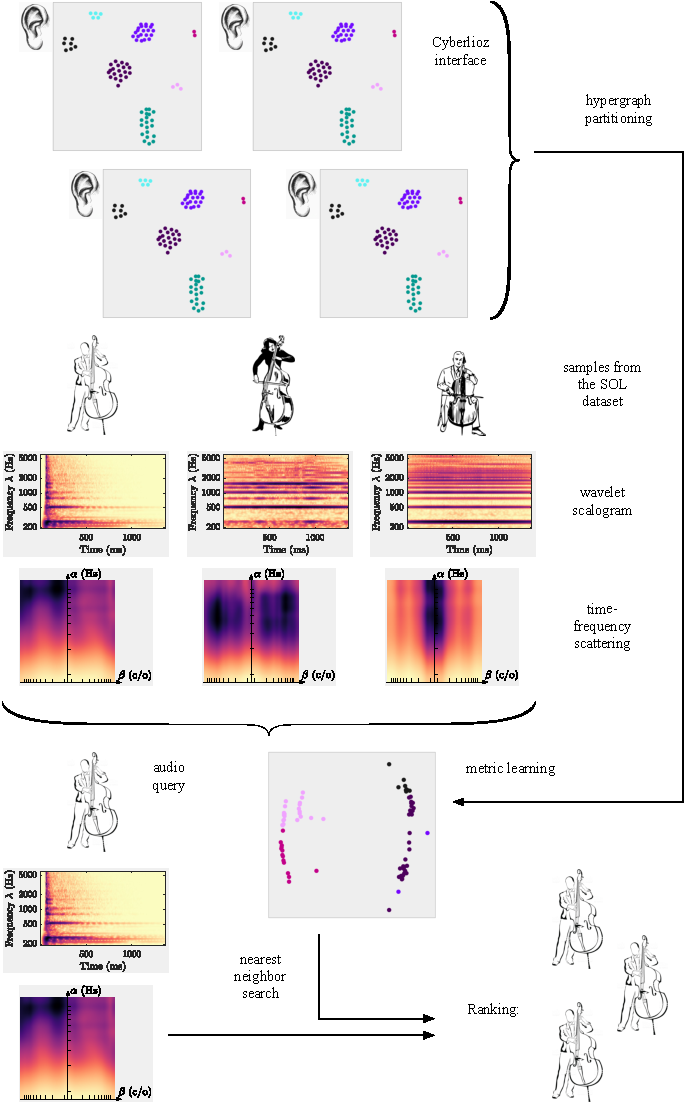
\includegraphics[width=0.9\textwidth]{figures/lostanlen2020jasmp_fig1_v3.pdf}
\caption{\csentence{Overview of the proposed approach}}
\label{fig:pipeline}
\end{figure}
\clearpage

\subsection*{Outline}
The \lnameref{sec:soa} section reviews recent research in the computational modeling of musical timbre.
The \lnameref{sec:survey} section describes our data collection procedure for auditory similarities across playing techniques.
The \lnameref{sec:method} section presents the technical components of our machine listening system, namely joint time--frequency scattering and large-margin nearest neighbors.
The \lnameref{sec:results} section conducts an ablation study of our system.
The \lnameref{sec:discussion} section summarizes the implications of our findings for future research on timbral similarity.\footnote{Reproducible research statement: the implementation of the proposed model and the experimental protocol of this paper are available online, alongside anonymized data from human subjects:  \url{https://github.com/mathieulagrange/paperPlayingTechniquesSimilarityLearning}} %TODO: simplify this URL to lostanlen2020jasmp





\section*{\nmu Related work}
\label{sec:soa}

Timbre involves multiple time scales in conjunction, from a few microseconds for an attack transient to several seconds for a sustained tone.
Therefore, computational models of timbre perception must summarize acoustic information over a long analysis window, typically amounting to $10^{4}$ digital audio samples or more \cite{joder2009taslp}.
Mapping this input to a feature space in which distances denote timbral dissimilarities requires a data-driven stage of dimensionality reduction.
In this respect, the scientific literature exhibits a methodological divide as regards the collection of human-annotated data \cite{siedenburg2016jnmr}.


\subsection*{Timbre modeling in music information retrieval (MIR)}
On the one hand, most publications in music information retrieval cast timbre modeling as an audio classification problem  \cite{martin1998asa,brown1999jasa,eronen2000icassp,herrera2003jnmr,wieczorkowska2003jiis,livshin2004dafx,krishna2004icassp,kaminskyj2005jiis,benetos2006icassp,bhalke2016jiis}.
In this context, the instrumentation of each musical excerpt serves as an unstructured set of ``audio tags,'' encoded as binary outputs within some predefined label space.
Because such tags often belong to the metadata of music releases, the process of curating a training set for musical instrument classification requires little or no human intervention.
Although scraping user-generated content from online music hosting platforms may not always reflect the true instrumentation with perfect accuracy, it offers a scalable and ecologically valid insight onto the acoustic underpinnings of musical timbre.

Furthermore, supplementing user-generated content with the outcome of a crowdsourced annotation campaign allows an explicit verification of instrument tags.
For instance, the Open-MIC dataset \cite{humphrey2018ismir}, maintained by the Community for Open and Sustainable Music Information Research (COSMIR) \cite{mcfee2016ismir}, comprises a vast corpus of 20k polyphonic music recordings spanning 20 instruments as a derivative of the Free Music Archive (FMA) dataset \cite{defferrard2017ismir}.
Another example is the Medley-solos-DB dataset \cite{lostanlen2016ismir}, which comprises 21k monophonic excerpts from 8 instruments as a derivative of the MedleyDB dataset of multitrack music \cite{bittner2014ismir}.

Over the past decade, the availability of large digital audio collections, together with the democratization of high-performance computing on dedicated hardware, has spurred the development of deep learning architectures, and notably deep convolutional networks, in music instrument recognition \cite{mcfee2015ismir,pons2017eusipco,gururani2018ismir}.
Notwithstanding the growing accuracy of these architectures in the large data regime, it remains unclear how to extend them from musical instrument recognition to playing technique recognition, where labeled samples are considerably scarcer.
We refer to \cite{han2017taslp} for a recent review of the state of the art in this domain.


\subsection*{Timbre modeling in music cognition research}
On the other hand, the field of music psychology investigates timbre with the aim of discovering its physiological and behavioral foundations \cite{mcadams2009chapter}.
In this setting, prior knowledge, however accurate, of instrumentation does not suffice to conduct a study.
Rather, each excerpt must be played back to multiple human listeners.
Yet, collecting subjective responses to acoustic stimuli is a tedious and unscalable procedure, restricting the size of the musical corpus under study.
Such restriction hampers the applicability of iterative representation learning algorithms, such as stochastic gradient descent in deep neural networks.
Nevertheless, while training artificial neurons is prone to statistical overfitting, advanced methods in electrophysiology allow to observe the firing patterns of biological neurons in the presence of controlled stimuli.
This observation, originally carried out on the ferret, has led to a comprehensive mapping of the primary auditory cortex in terms of its spectrotemporal receptive fields (STRFs) \cite{depireux2001jneur}, thus yielding a useful form of inductive bias for downstream machine listening applications.

The STRF of a neuron is a function of time and frequency which represents the optimal predictor of its post-stimulus time histogram (PSTH) during exposure to a diverse range of auditory stimuli \cite{aertsen1981biolcyb}.
The simplest method to compute it in practice is by reverse correlation, i.e.\ by averaging all stimuli that trigger an action potential \cite{deboer1968biomed}.
Historically, STRFs were defined by their Wigner--Ville distribution \cite{flandrin1998book}, thereby sparing the choice of a tradeoff in time--frequency localization, but eliciting cross-term interferences \cite{eggermont1993hearing}.
Since then, the STRF of a neuron was redefined as a spectrographic representation of its spike-triggered average \cite{klein2000compneur}.
Although this new definition is necessarily tied to a choice of spectrogram parameters, it yields more interpretable patterns than a Wigner--Ville distribution.
In particular, a substantial portion of spectrographic STRFs exhibits a ripple-like response around a given region $(t, \lambda)$ of the time--frequency domain \cite{theunissen2000jneur}.
This response can be approximately described by a pair of scalar values: a temporal modulation rate $\alpha$ in Hertz and a frequential modulation rate $\beta$ in cycles per octave.

Interestingly, both $\alpha$ and $\beta$ appear to be arranged in a geometric series and independent from the selected center time $t$ and center frequency $\lambda$.
This observation has led auditory neuroscientists to formulate an idealized computational model for STRF, known as ``full cortical model'' \cite{chi2005jasa}, which densely covers the rate--scale domain $(\alpha, \beta)$.


\subsection*{Spectrotemporal receptive fields (STRF)}
Over recent years, several publications have employed the full cortical model as a feature extractor for a task of musical instrument classification, both in isolated recordings \cite{patil2012ploscompbiol} and in solo phrases \cite{patil2015eurasip}.
These biologically inspired features outperform the state of the art, especially in the small data regime where deep learning is inapplicable.
Furthermore, the confusion matrix of the full cortical model in the label space of musical instruments strongly correlates with the confusion matrix between a human listener and the ground truth.
Another appeal of the full cortical model is that the third-order $(\lambda, \alpha, \beta)$ tensor of frequencies, rates, and scales can be segmented into contiguous regions of maximal perceptual relevance for each instrument \cite{thoret2016jasa}.
This is unlike fully end-to-end learning architectures, whose post hoc interpretability requires advanced techniques for feature inversion \cite{mishra2018ismir}.
Lastly, beyond the realm of supervised classification, a previous publication \cite{hemery2015frontiers} has shown that query-by-example search with STRFs allows to discriminate categories of environmental soundscapes, even after temporal integration and unsupervised dimensionality reduction.

The reasons above make STRFs an appealing feature extractor for a perceptual description of timbral similarity across instrumental playing techniques.
Nonetheless, current implementations of STRF suffer from a lack of scalability, which explains why they have found few applications in MIR thus far.
Indeed, the full cortical model is usually computed via two-dimensional Fourier transforms over adjacent time--frequency regions, followed by averaging around specific rates and scales.
On the contrary, joint time--frequency scattering offers a faster extraction of spectrotemporal modulations while preserving properties of differentiability \cite{andreux2019jmlr} and invertibility \cite{lostanlen2019dafx}.
Such acceleration is made possible by discretizing the wavelet transforms involved in time--frequency scattering according to a multirate scheme, both along the time and the log-frequency variables \cite{anden2019tsp}.
This multirate scheme also has the benefit of drawing an explicit connection between scattering networks and deep convolutional networks, as both involves numerous convolutions with small kernels, pointwise rectifying nonlinearities, and dyadic pooling operations \cite{mallat2016philtrans}.

Moreover, a quantitative benchmark over Medley-solos-DB has demonstrated that joint time--frequency scattering, unlike purely temporal scattering, outperforms deep convolutional networks in supervised musical instrument classification, even in a relatively large data regime with 500 to 5k samples per class \cite{anden2019tsp}.
Recently, Wang et al.~\cite{wang2019ismir} trained a classifier of playing techniques on separable (\ie{} non-joint) time--frequency scattering features \cite{anden2014tsp}, and achieved state-of-the-art results in continuous performance recordings of the Chinese bamboo flute. % TODO cite wang 2020 icassp
Despite supplying experimental evidence that time--frequency scattering is better suited to playing technique recognition than purely temporal scattering, it remains to be seen whether these findings can scale up from a single instrument to an entire orchestra.
In addition, previous publications in time--frequency scattering, whether separable or joint, lack a human-centric evaluation, independently from any classification task.

\subsection*{Claim of originality}
The contributions of this paper strive to fill the gap in scholarship between MIR and music cognition approaches to timbre, in the context of computer-assisted spectralist orchestration with extended playing techniques.
From the standpoint of MIR, the model presented here offers a tractable and generic multidimensional representation for timbre similarity, alongside formal guarantees of robustness to elastic deformations in the time--frequency domain.
Conversely, from the standpoint of music cognition, our model offers a scalable and biologically plausible surrogate for stimulus-based collection of acoustic dissimilarity judgments, with the potential of being readily tailored to subjective preferences.


% enjoys a thirty-fold reduction in dimensionality, while covering a  time span that is four times larger (1000 ms) and an acoustic bandwidth that is also four times larger (0--16 kHz).
%We refer to \cite{bellet2015book} for a review of the state of the art in metric learning.

\section*{\nmu Timbre similarity judgments}
\label{sec:survey}

The European symphonic orchestra encompasses four families of instruments: strings, woodwinds, brass, and percussion.
In this article, we focus on the former three, and leave the question of learning auditory similarities between percussion instruments to future research.
The reason behind this choice is that most percussive instruments do not allow much variation in terms of pitch or intensity, if at all; thus reducing the amount of intra-technique variability in the time--frequency domain.
Furthermore, although percussive instruments certainly exhibit a rich diversity of playing techniques (we refer to \cite{peinkofer1976book} for a survey) these are rarely shared with pitched instruments.
In comparison, techniques for sustained tones such as \emph{vibrato} or \emph{tremolo} permeate throughout a vast instrumentarium, \eg{} bowed strings and reed alike.
We refer to \cite{wu2018taslp} and \cite{pearce2019appliedsciences} for reviews of the recent literature on the timbre modeling of percussive instruments, from the standpoints of MIR and music cognition respectively.

\subsection*{Dataset}
We consider a list of 16 instruments: violin (Vn), viola (Va), cello (Vc), contrabass (Cb), concert harp (Hp), Spanish guitar (Gtr), accordion (Acc), flute (Fl), soprano clarinet (BbCl), alto saxophone (ASax), oboe (Ob), bassoon (Bn), trumpet in C (TpC), French horn (Hn), tenor trombone (TTbn), and bass tuba (BBTb).
Among this list, the former six are strings, the next six are woodwind, and the last four are brass.
Some of these instruments may be temporarily equipped with timbre-altering mutes, such as a rubber sordina on the bridge of a violin or an aluminium ``wah-wah'', also known as \emph{harmon}, inside in the bell of a trumpet.
Once augmented with mutes, the list of 16 instruments grows up to 33.
Furthermore, every instrument, whether equipped with a mute or not, affords a panel of playing techniques ranging in size between 11 (for the accordion) and 41 (for the bass tuba).
In the rest of this paper, we abbreviate instrument--mute--technique by means of the acronym ``IMT''.
One example of IMT is \texttt{TpC+S-ord}, \ie{} trumpet in C with a straight mute played in the ordinary technique.
Another example of IMT is \texttt{Vn-pont}, \ie{} violin without any mute played in the \emph{sul ponticello} (bowing near the bridge) technique.

Performers can play each IMT at various pitches, according to a tessitura that depends on the instrument but not on the choice of mute.
Among the 16 instruments in this study, the two instruments with widest and narrowest tessituras, in their respective ordinary techniques, are the accordion (81 semitones) and the trumpet in C (32 semitones) respectively.
Lastly, each IMT may be played at up to five intensity dynamics, ranging from quietest to loudest as: pianissimo (\emph{pp}), piano (\emph{p}), mezzo forte (\emph{mf}), forte (\emph{f}), and fortissimo (\emph{ff}).
However, the resort to a non-ordinary playing technique may restrict both the tessitura and the dynamics range of the instrument--mute pair under consideration.
For example, the pitch of pedal tones in brass instruments is tied to the fundamental mode of the bore, \ie{} usually B-flat or F. % TODO check this, use special package for musical pitches
Likewise, the intensity of key clicks in the oboe is necessarily \emph{pp}, while the intensity of snap pizzicato \emph{\`a la Bart\'ok} in plucked strings is necessarily \emph{ff}.

In summary, audio signals from isolated musical notes may vary across three categorical variables (instrument, mute, and technique) and two continuous variables (intensity and pitch).
The Cartesian product of all five variables results in a combinatorial explosion of possible timbral sensations.
The Studio On Line dataset (SOL), recorded at Ircam in 1998, offers a dense sampling of this combinatorial explosion, amounting to 25444 audio signals in total.
We should note that this dense sampling is by no means comprehensive, as it erases other factors of acoustic variability, such as identity of performer, identity of instrument manufacturer, audio acquisition equipment, and room response characteristics; which are all restricted to singletons.
Addressing these factors of variability is besides the scope of this paper, which focuses on the influence of playing technique.
Despite this deliberate restriction, the size of the SOL dataset remains impractically large for collecting human similarity judgments.
Our protocol addresses this problem by means of three complementary approaches: disentanglement of factors, expert pre-screening, and efficient annotation interface.

\subsection*{Disentanglement of factors}
First, we purposefully disentangle categorical variables (IMTs) from continuous variables (pitch and intensity) in the SOL dataset.
Indeed, under first approximation, the perception of timbre is invariant to pitch and intensity.
Therefore, we select auditory stimuli according to a reference pitch and a reference intensity; in our case, middle C (\ie{} C4) and \emph{mf}. % TODO use pitch spelling package
After this selection, every IMT triplet contains a single acoustic exemplar, regarded as canonical in the following.
The number of canonical stimuli for the entire SOL dataset is equal to 235.
We should note, however, that the proposed pitch--intensity cannot be strictly enforced across all IMTs.
Indeed, as explained above, a fraction of IMTs can only be achieved at restricted values of pitch and intensity parameters, \eg{} pedal tones or key clicks.
Therefore, at a small cost of consistency, we only enforce the pitch--intensity reference (\ie{} C4 and \emph{mf}) when practically feasible, and fall back to other pitches and intensities if necessary.


\subsection*{Expert pre-screening}
Secondly, we reduce the number of IMTs in our study by focusing on those which are deemed to be most relevant.
Here, we define the relevance of an IMT as the possibility of imitating it by means of another IMT from a different instrument.
One example of such imitation is the acoustic similarity between slap tonguing in reed instruments and a snap pizzicato in strings instruments.
To collect perceptual ratings of relevance, we recruited two professors in music composition at the Paris Conservatory (CNSMDP), and explicitly gave them our definition of relevance.
Each of them inspected the entire corpus of $235$ IMTs and annotated them in terms of relevance according to a Likert scale with seven ticks.
In this Likert scale, the value 1 (least relevant) denotes that the IMT under consideration has a timbre that is idiosyncratic of the instrument, and that therefore, it is unlikely that humans will pair it with IMTs from other instruments.
Conversely, the value 7 (most relevant) denotes that the IMT under consideration has a strong similarity with IMTs from one or several other instruments.

Once both experts completed their annotation, we retained all IMTs whose average relevance score was judged equal to 3 or higher.
At the end of this stage of pre-screening, the list of IMT reduces from 235 to $N=78$.
Tables 1 and 2, in the Appendix section of this paper, give a full list of these 78 highly relevant IMTs.
It is worth noting that, according to both experts, the timbre of the accordion was judged too idiosyncratic, regardless of playing technique, to be relevant for this experiment.
Indeed, the accordion is the only instrument in the aforementioned list of 
instrument to have free reeds, keyboard-based actuation, or handheld airflow.
Consequently, regardless of mute and technique, the set of instruments $\mathcal{I}$ in our study contains 15 elements.

\subsection*{Efficient annotation interface}
Thirdly, we design a graphical user interface for partitioning a corpus of short audio samples.
The need for such an interface arises from the unscalability of Likert scales in the context of pairwise similarity judgments.
Assuming that similarity is a symmetric quantity, collecting a dense matrix of continuously valued ratings of similarity among a dataset of $N$ items would require $\frac{1}{2}(N^2-N)$ Likert scales.
In the case of $N=78$ IMTs, the task would amount to about 3k horizontal sliders, \ie{} several hours of cumbersome work for the human annotator.
Engaging as many participants as possible in our study called for a more streamlined form of human--computer interaction, even if it sacrificed the availability of continuous ratings.
To this end, we implemented a web application, named Cyberlioz, in which the user can spontaneously listen and arrange sounds into clusters of timbre similarity\footnote{The Web application for efficient audio annotation, as well as the raw anonymized responses of all $31$ participants to our study, is available at: \url{https://soundthings.org/research/cyberlioz/}}.
The name Cyberlioz is a portmanteau between the prefix cyber- and the French composer Hector Berlioz.
The choice is by no means coincidental: Berlioz is famous for having, in his \emph{Treatise on Orchestration} (1844), shed a particular focus on the role of timbre as a parameter for musical expression.
 
 
Cyberlioz consists of a square panel on which is displayed a collection of circular grey dots, each of them corresponding to one of the $N=78$ IMTs, and initially distributed uniformly at random.
Hovering the screen pointer onto each dot results in a playback of a representative audio sample of this IMT, \ie{} C4 and \emph{mf} in most cases. % TODO VL: use pitch notation library to express C4
Furthermore, each dot can be freely placed on the screen by clicking, dragging, and dropping.
Lastly, the user can assign a color to each dot by selecting it among a palette of 20 hues.
The goal of the Cyberlioz interface is to form clusters of timbre similarity between IMTs, expressed by sameness of color.
Here, any two audio samples are defined as similar if and only if one can be replaced by the other in a context of spectralist orchestration.

In comparison with a traditional Web-based form, Cyberlioz offers a more intuitive and playful user experience, while expediting the obtention of a dense matrix ($N\times N$) of similarity judgments within a moderate duration of $30$ to $60$ minutes for each participant.
In X 2016, we recruited volunteers to use Cyberlioz on their own computers, via a web browser, and equipped with a pair of earphones. % TODO give the exact two months.
We publicized this study on international mailing lists for research in music audio processing, such as X and Y. % TODO give mailing lists
Within two months, $K=31$ subjects accessed Cyberlioz and completed the task. % TODO break down by gender? give age stats? musical experience?
%Figure \ref{fig:xp2display}. % TODO

\subsection*{Hypergraph partitioning}
Once the data collection campaign was complete, we analyzed the color assignments of each subject $k$ and converted them into a similarity graph $\mathcal{G}_k$, where the integer $k$ is an anonymized subject index, ranging between $1$ and $K$.
For a given $k$, the graph $\mathcal{G}_k$ contains $N=78$ vertices, each representing a different IMT in the corpus.
In $\mathcal{G}_k$, an edge connects any two vertices $m$ and $n$ if the corresponding dots in Cyberlioz have the same color.
Otherwise, there is no edge connecting $m$ and $n$.
This way, $\mathcal{G}_k$ contains as many connected components as the number of similarity clusters for the subject $k$, \ie{} the number of distinct colors on the Cyberlioz interface in the response of $k$.

%Only the clustering given by the subjects using the color labels is considered to estimate the spontaneous judgments of similarity among \ipt. The spatial organization of the dots representing the \ipt could provide information about the similarity, but this would implicitly enforce the fact that the timbral similarity space is two dimensional. We therefore now only study the properties of the clusterings performed by the subject prior to converting them into an overall similarity matrix.

We aggregate the similarity judgments from all $K$ subjects by embedding them into a hypergraph $\mathcal{H}$, that is, a graph whose edges may connect three or more vertices at once.
Specifically, $\mathcal{H}$ contains $N$ vertices, each representing an IMT; and each ``hyperedge'' in $\mathcal{H}$ corresponds to some connected component in one of the graphs $\mathcal{G}_k$'s among all subject $k$.
Then, we convert the hypergraph $\mathcal{H}$ back into a conventional graph $\mathcal{G}_0$ by means of a combinatorial optimization algorithm algorithm known as hypergraph partitioning \cite{kernighan1970efficient,han1997scalable,strehl2002cluster}. % TODO describe the gist of hypergraph partitioning?
To construct $G_0$, we select a number of clusters $C=5$ a priori, and run hypergraph partitioning to assign each vertex $i$ to one of these clusters.
Intuitively, hypergraph partitioning optimizes a tradeoff between two objectives: first, balancing the size of all clusters in terms of their respective numbers of vertices; and secondly, keeping most hyperedges enclosed within as few distinct clusters as possible.

While the graphs $\mathcal{G}_1 \ldots \mathcal{G}_K$ encode the subjective similarity judgments of participants $1$ to $K$, the graph $\mathcal{G}_0$ represents a form of consensual judgment that is shared across all participants, while discarding intersubjective variability.
Although the rest of our paper focuses on the consensus $\mathcal{G}_0$, it is worth pointing out that the same technical framework could apply to a single subject $k$, or to a subgroup of the $K=31$ subjects.
This remark emphasizes the potential of our similarity learning method as a customizable tool for visualizing and extrapolating the timbre similarity space of a newcoming subject, after less than one hour of using Cyberlioz.


\subsection*{Inter-instrument similarity}

Before addressing the question of modeling timbre in the audio domain, we conduct an exploratory study on the structure of similarity judgments themselves.
Specifically, we ask whether human listeners, when confronted with a diverse corpus of IMT samples, tend to cluster those samples in terms of an organological taxonomy.
To answer this question, we derive from the consensus clustering graph $\mathcal{G}_0$ an instrument-wise similarity matrix $\mathbf{A}_{\mathcal{I}}$ whose rows and columns are defined on the finite set $\mathcal{I}$ of instruments.
For every instrument--instrument pair $(i,j)$, we set the value of $\mathbf{A}_{\mathcal{I}}$ at row $i$ and column $j$ equal to the number of pairs in $\mathcal{G}_0$ from instruments $i$ and $j$ respectively, renormalized by the number of IMT samples from either instrument $i$ or instrument $j$:
\[
\mathbf{A}_{\mathcal{I}}(i,j) = \dfrac{
2\,\Card \big\{ (m, n) \,\vert\, \mathrm{Instrument}(m)=i ; \mathrm{Instrument}(n)=j ; m \overset{\mathcal{G}_0}{\sim} n \big\}
}{
\Card \big\{n \,\vert\, \mathrm{Instrument}(n) \in \{ i, j \} \big\}
}.
\label{eq:instrument-similarity}
\]

Then, we run Ward's method to cluster instruments in $\mathcal{I}$ according to the similarity matrix $\mathbf{A}_{\mathcal{I}}$.
This method yields a permutation $\sigma_{\mathcal{I}}: \mathcal{I} \rightarrow \mathcal{I}$ of the rows and columns in $\mathbf{A}_{\mathcal{I}}$.
Intuitively, for every instrument--instrument pair $(i, j) \in \mathcal{I}^2$, the distance $\vert \sigma_{\mathcal{I}}(i) - \sigma_{\mathcal{I}}(j) \vert$ after permutation is small if and only if the similarity $\mathbf{A}_{\mathcal{I}}(i, j)$ is large.
Figure \ref{fig:consensusVsI} displays the rearranged similarity matrix $\widetilde{\mathbf{A}}_{\mathcal{I}} : (i,j)\in \mathcal{I}^2 \mapsto \mathbf{A}_{\mathcal{I}}(\sigma_{\mathcal{I}}^{-1}(i), \sigma_{\mathcal{I}}^{-1}(j))$ as a result of such agglomerative hierarchical clustering procedure.

Interestingly, the matrix $\widetilde{\mathbf{A}}_{\mathcal{I}}$ exhibits a block diagonal structure, which roughly reflects the classical taxonomy of musical instruments: four woodwinds (BbCl, Fl, ASax, Ob) are clustered together, followed by a cluster containing one woodwind (Bn) and four brass (BBTb, Hn, TTbn, and TpC), followed by a cluster of all strings (Cb, Va, Vn, Vc, Gtr, Hp).
Furthermore, the largest cross-instrument similarity arises for the only pair of purely plucked instruments, namely, harp and guitar.

\begin{figure}
\center
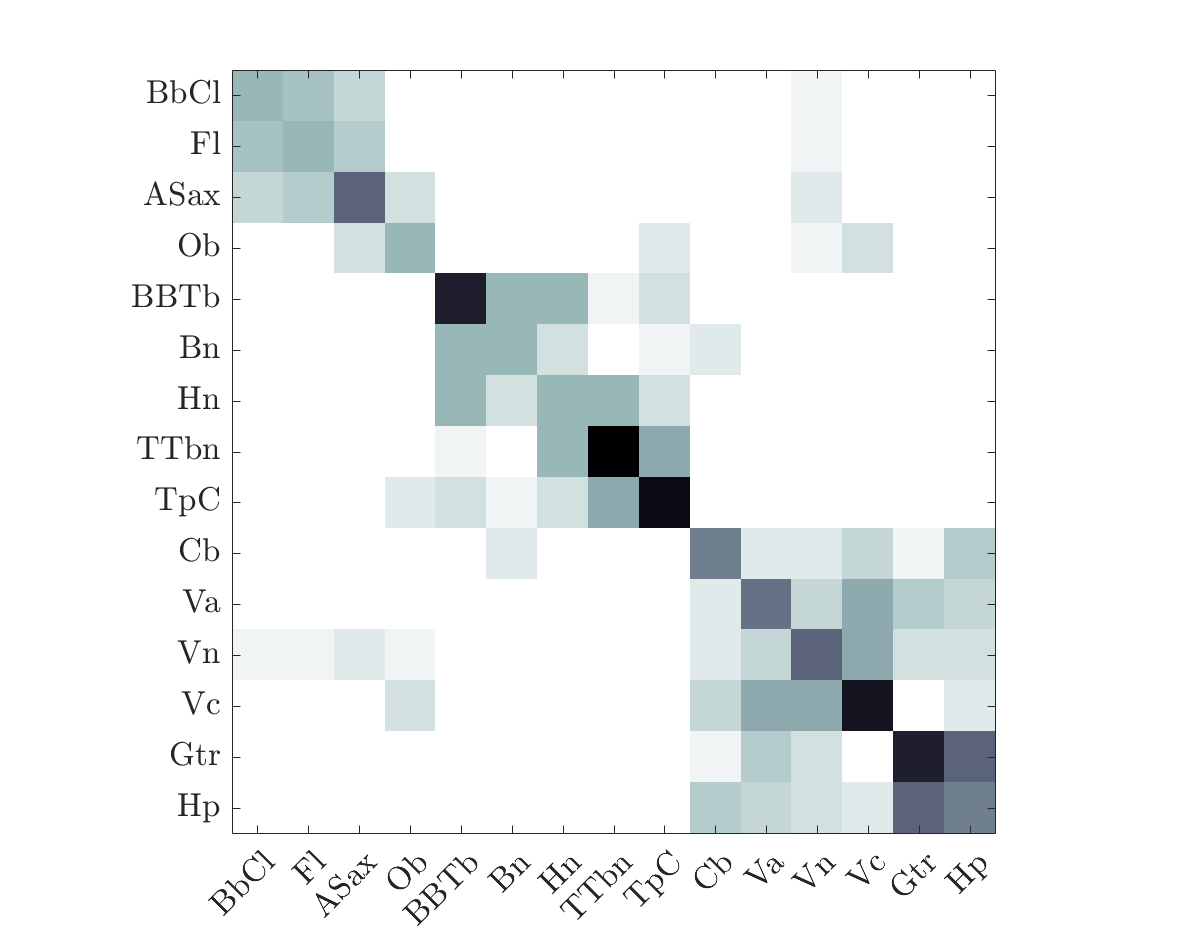
\includegraphics[width = \textwidth]{figures/consensusVsI.png}
\caption{
%TODO caption
}
\label{fig:consensusVsI}
\end{figure}


\subsection*{Inter-technique similarity}
From the consensus clustering graph $\mathcal{G}_0$, we also derive a technique-wise similarity matrix $\mathbf{A}_{\mathcal{T}}$ whose rows and columns are defined on the finite set $\mathcal{T}$ of playing techniques.
We define the similarity between any two playing techniques $u$ and $v$ in $\mathcal{T}$ as the following ratio of set cardinals:
\[
\mathbf{A}_{\mathcal{T}}(u,v) = \dfrac{
2\,\Card \big\{ (m, n) \,\vert\, \mathrm{Technique}(m)=u ; \mathrm{Technique}(n)=v ; m \overset{\mathcal{G}_0}{\sim} n \big\}
}{
\Card \big\{n \,\vert\, \mathrm{Technique}(n) \in \{ u, v \} \big\}
},
\]
alike the definition of $\mathbf{A}_{\mathcal{I}}$.
Again, we run Ward's method to cluster playing techniques in $\mathcal{T}$ according to their similarity $\mathbf{A}_{\mathcal{T}}$.
Figure \ref{fig:consensusVsPt} displays the rearranged similarity matrix $\widetilde{\mathbf{A}}_{\mathcal{T}} : (u,v)\in \mathcal{T}^2 \mapsto \mathbf{A}_{\mathcal{T}}(\sigma_{\mathcal{T}}^{-1}(u), \sigma_{\mathcal{T}}^{-1}(v))$ as a result of such agglomerative hierarchical clustering procedure.

Contrary to inter-instrument similarity (Figure \ref{fig:consensusVsI}), inter-technique similarity does not exhibit a clear segregation of instrument families.
For example, the first two rows in $\widetilde{\mathbf{A}}_{\mathcal{T}}$ correspond to a oboe sample (\texttt{Ob-blow-no-reed-C4}, \ie{} blowing without the reed) and a cello sample (\texttt{Vc-legno-tratto-C4-mf-1c}, \ie{} drawing the wooden part of the bow across the string) respectively, despite the fact that the oboe is a woodwind instrument whereas the cello is a string instrument.

More generally, even though the block diagonal structure of the matrix $\widetilde{\mathbf{A}}_{\mathcal{T}}$ is less prevalent than in $\widetilde{\mathbf{A}}_{\mathcal{I}}$, playing technique clusters appear to transcend instrument categories.
Nevertheless, these clusters correspond to some basic attributes of qualitative timbre: by and large, the top-left region of the matrix contains sustained sounds whereas the bottom-right region contains percussive sounds.
Interestingly, the ordinary technique (\texttt{ord}) appears at the center of the matrix, \ie{} at the intersection between sustained sounds and percussive sounds.
This is because the notion of ``ordinariness'' does not prescribe the same gesture for all instruments: \eg{}, an ordinary guitar sound is expected to be percussive whereas an ordinary flute sound is expected to be sustained.


\begin{figure}
\center
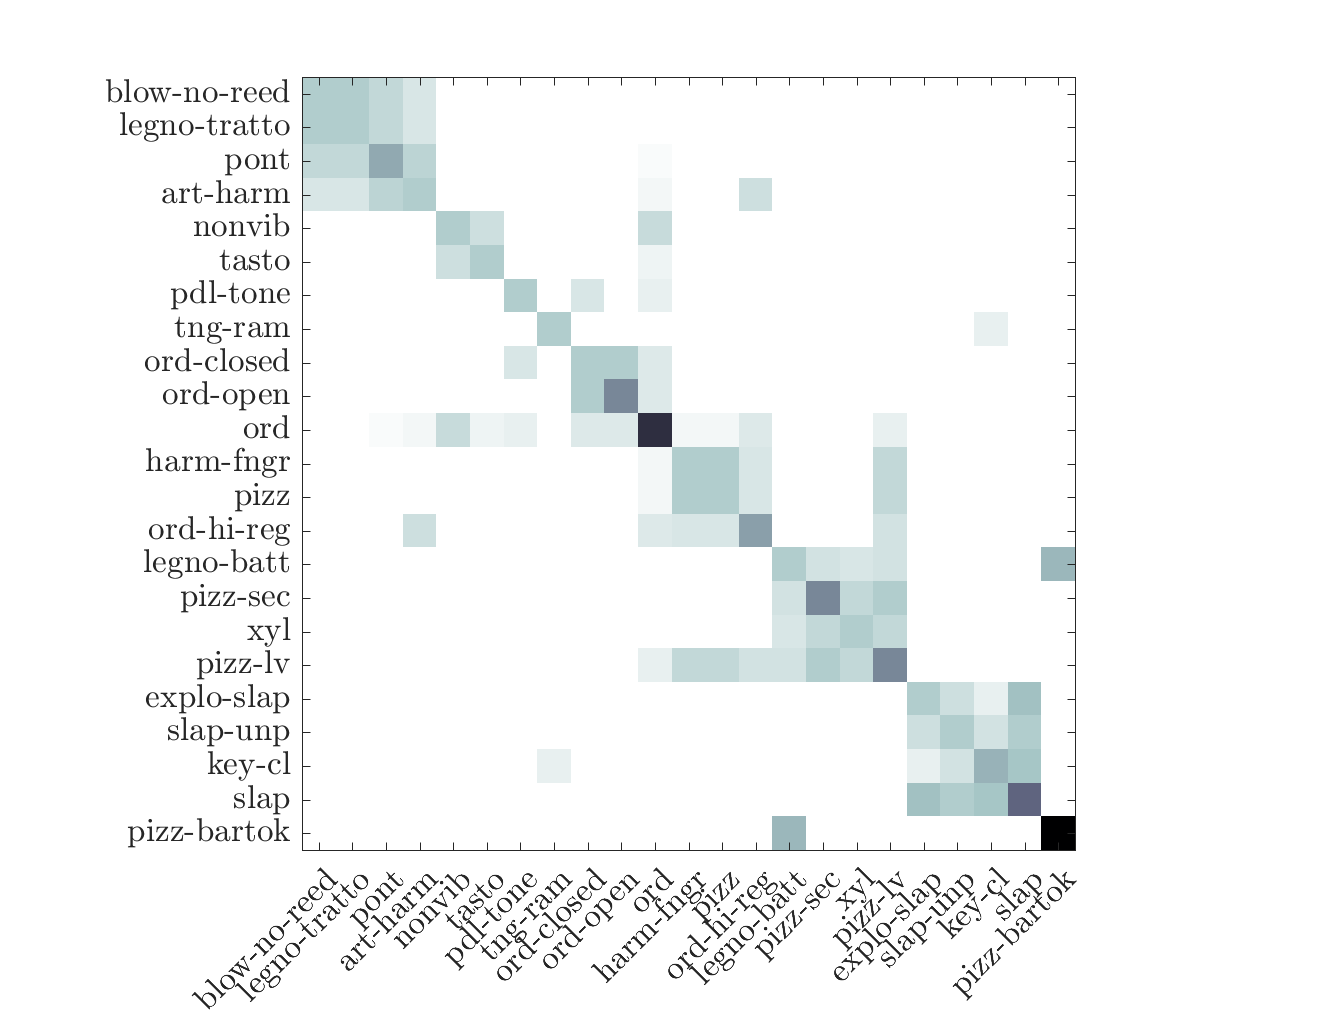
\includegraphics[width = \textwidth]{figures/consensusVsPt.png}
\caption{A description of the playing technique abbreviations in made available in the Appendix (Tables \ref{tab:list1} and \ref{tab:list2}).
%TODO add a double arrow
% rough <-- soft --> rough
% sustained <-- "ordinary" --> percussive
}
\label{fig:consensusVsPt}
\end{figure}



\section*{\nmu Methods}
\label{sec:methods}
The previous section described our protocol for collecting timbral similarity judgments between instrumental playing techniques at scale.
In this section, we aim to recover these similarity judgments from digital audio recording, according to a paradigm of supervised metric learning.
To this end, we present a new machine listening system, composing joint time--frequency scattering and large-margin nearest neighbors (LMNN).

%Following the above discussed matters, we propose a ranking system that is based on a processing pipeline made of two main components, see Figure \ref{fig:pipeline}.
%The first component maps the audio signal of the query and the items of the database into a high-dimensional timbre space using the scattering transform.
%The second component warps this timbre space by taking into account perceptual judgments represented as a consensus clustering of the items in the dataset, as presented in the \nameref{sec:survey} section.
%This warping, or reweighting, of the space is performed using LMNN.


\subsection*{Joint time--frequency scattering transform}
\label{sec:scattering}

While cortical representations have been successful in distinguishing properties of audio recordings (including similarity analysis and classification tasks), they remain models for the electrophysiological signals recorded in the audio cortex.
As such, their calculation is not always computationally efficient and their mathematical properties may be difficult to analyze directly.

A closely related representation is that of the time scattering transform, introduced by And\'{e}n and Mallat \cite{anden2011multiscale,anden2014tsp}.
Given an audio recording, it decomposes the signal using an analytic wavelet transform and computes the modulus, obtaining the \emph{scalogram} of the signal.
The scalogram is similar to the spectrogram, but has a time--frequency resolution that varies with frequency: at low frequency, the filters are narrowly tuned in frequency (and hence wide in time), while at high frequency, the filters are wide in frequency (and hence narrowly concentrated in time).
This representation contains a large amount of information, but not in a form suitable for building statistical models.
In particular, the scalogram is not \emph{stable} in the sense that small deformations to the original signal may induce large changes to the scalogram.
It also lacks \emph{invariance} to time-shifting, which does not affect our perception of a sound, and should therefore not affect its timbre model.
One way to resolve this is to average the scalogram in time to obtain a spectral profile of the signal, yielding the first-order scattering coefficients.
These possess both invariance to time-shifting and stability to time-warping deformations \cite{anden2014tsp}.

Since these first-order coefficients only include spectral information, they cannot accurately characterize more sophisticated structure in the signal.
One way to augment them is to calculate another wavelet decomposition in time, this time on each frequency channel of the scalogram.
Again, we compute the modulus of the wavelet coefficients and average in time.
The resulting coefficients are known as the second-order time scattering coefficients.
These also possess the desired invariance and stability properties, but capture more information on the temporal structure of the scalogram \cite{anden2014tsp}.

While richer than a simple spectral decomposition, such as MFCCs, the second-order time scattering coefficients described above primarily capture structure in time.
Indeed, they do not explicitly encode frequency structure in an invariant and stable manner.
If a signal is transposed or warped in frequency by a small amount, we do not expect its timbre to change significantly.
We would therefore like our representation to have the same invariance and stability properties along the frequency axis.
This is achieved by taking first- and second-order scattering coefficients and computing a second scattering transform, this time along the log-frequency axis.
The resulting coefficients are known as separable time and frequency scattering coefficients \cite{anden2014tsp}.

This representation does possess the desired invariance and stability properties, but its separable nature limits its power to adequately represent time--frequency structures that do not separate cleanly in time and frequency, such as chirps.
To remedy this, another approach was suggested by And\'{e}n et al. \cite{anden2015mlsp,anden2019tsp} wherein the temporal wavelet decomposition of the scalogram is replaced with a two-dimensional, spectro-temporal decomposition.
Similarly to the cortical representation, the result is a four-dimensional array indexed by time, acoustic frequency, modulation frequency (or \emph{rate}), and spectral modulation frequency, known as \emph{quefrency} (or \emph{scale}).
As before, we compute the modulus and average in time, obtaining a set of coefficients known as second-order joint time--frequency scattering coefficients.

The definition of the scattering transform in terms of wavelet decompositions and modulus nonlinearities presents several advantages.
On the computational side, the critical bandwidth guarantees of wavelet transforms allows us to judiciously subsample the output, resulting in a lower-dimensional representation compared to the cortical representations.
The scattering transform also satisfies the aforementioned stability conditions, providing a guarantee that slightly deforming a signal only results in a negligible change in its scattering transform.
Furthermore, we may calculate the scattering transforms of several model signals, including amplitude-modulated harmonic sounds and noise excitations \cite{anden2012scattering,anden2014tsp}, frequency-modulated sinusoids (e.g., chirps) \cite{anden2012scattering,anden2019tsp}, and beating phenomena \cite{anden2014tsp}.
They have also enjoyed success in several audio classification and similarity retrieval tasks \cite{anden2011multiscale,bauge2013representing,anden2014tsp,anden2019tsp,lostanlen2018jasmp,lostanlen2018extended}.
%\ja{Need to flesh out the above with some equations.
%We're no longer talking to biologists, so we don't need to be afraid.}
% TODO: avoid citing the same papers over and over


\ml{VL. provide parameters for scattering
\texttt{
case 'scat'
    filt\_opt.Q = [12 1];
    filt\_opt.J = T\_to\_J(sr*setting.sct/1000, filt\_opt);
case 'tfscat'
    tm\_filt\_opt.Q = [12 1];
    tm\_filt\_opt.J = T\_to\_J(sr*setting.sct/1000, tm\_filt\_opt);
    fr\_filt\_opt.J = 4;}}

\begin{figure}
\caption{\csentence{Sample scattering}
Same 3 sounds spec + scatt.
% TODO figure + caption
}
\end{figure}

\subsection*{Metric learning with large-margin nearest neighbors (LMNN)}
\label{sec:weighting}

The standard Euclidean distance on the raw scattering coefficients provides an instrument-agnostic representation of timbre dissimilarity.
We now consider a transformation of this distance, in effect warping the timbre space, in order to more closely mimic a particular set of timbre similarity judgments.

Due to the size of corpus, we restrict ourselves to a simple linear transform of the scattering coefficients. More flexible and powerful methods could be brought to bear on this problem, such as deep neural networks, but with their flexibility comes an increase of the needed size of training data.

Specifically, we construct a positive semidefinite matrix $L$ that we apply to the scattering coefficients $x$ so that the Euclidean distance between $Lx$ and $Ly$ best approximates the consensus clustering obtained above.
We expect the resulting representation $Lx$ to provide a more accurate model for timbre perception.

We now use the consensus clustering to reweight the similarity between feature vectors (either MFCCs or scattering transforms).
For this, we use the \emph{large margin nearest neighbor} (LMNN) metric learning algorithm \cite{weinberger2006distance, weinberger2009distance}.
This approach constructs a positive semi-definite weighting matrix $L$ such that the distance $\|Lx - Ly\|$ best classifies a set of points into a fixed clustering assignment.
% TODO: this section needs more detail. In particular, it is worth discussing the role of Euclidean distances as an "initial guess" for LMNN. (this is unlike MLR, for example).
% cite Musgrave et al. Metric learning reality check

$\mathcal{Y}_1 (\boldsymbol{x}) = \mathcal{Y} \backslash \lbrace \boldsymbol{x} \rbrace$.

\begin{equation}
\mathbf{\Phi}_1 (\boldsymbol{x}) =
\arg \min_{\boldsymbol{y}\in \mathcal{Y}_1(\boldsymbol{x})}
\;
\big\Vert
\mathbf{L}\mathbf{\widetilde{S}}\boldsymbol{x}
-
\mathbf{L}\mathbf{\widetilde{S}}\boldsymbol{y}
\big\Vert
\end{equation}

$\mathcal{Y}_{r} (\boldsymbol{x}) = \mathcal{Y}_{(r-1)}(\boldsymbol{x}) \backslash \lbrace \mathbf{\Phi}_r (\boldsymbol{x}) \rbrace$.

\begin{equation}
\mathbf{\Phi}_r (\boldsymbol{x}) =
\arg \min_{\boldsymbol{y}\in \mathcal{Y}_r(\boldsymbol{x})}
\;
\big\Vert
\mathbf{L}\mathbf{\widetilde{S}}\boldsymbol{x}
-
\mathbf{L}\mathbf{\widetilde{S}}\boldsymbol{y}
\big\Vert
\end{equation}


\section*{\nmu Results}
\label{sec:results}

The previous section described our methods for extracting spectrotemporal modulations in audio signals, as well as learning a non-Euclidean similarity metric between them.
We now turn to apply these methods to the problem of allocating isolated musical notes to clusters of some timbre similarity graph $\mathcal{G}$.
In practice, for training purposes, the cluster graph $\mathcal{G}$ stems from the consensus of $K=31$ users of the Cyberlioz web application, which was described in the \lnameref{sec:survey} section ($\mathcal{G}=\mathcal{G}_0$).
However, for evaluation purposes, this cluster graph corrsponds to the subjective preferences of a single user $k$, in which case we take $\mathcal{G}=\mathcal{G}_k$.
% browsing a large-scale digital library of isolated musical notes, involving an extended vocabulary of playing techniques.

% TODO VL: organize design choices.
% (1) temporal support
% (2) time-frequency scattering / time scattering
% (3) learning / no learning



\subsection*{Semi-supervised label propagation}

In order to suit the practical needs of contemporary music composers, computer-assisted orchestration must withdraw from a diverge realm of instruments and techniques.
Therefore, whereas our data collection procedure for timbre similarity judgments focused on a single pitch (middle C) and a single intensity (\emph{mf}), we formulate our machine listening experiment on an expanded dataset of audio samples, containing variations in pitch and dynamics.

Given an audio stimulus $n$ from our perceptual study, we seek its position in the cluster graph $\mathcal{G}$.
Then, we identify its instrument--mute--technique (IMT) triplet, scrape for audio samples in SOL matching this triplet, and assign them all to the same cluster as the original audio stimulus.
We repeat the same procedure for all $N=78$ nodes in $\mathcal{G}_0$, resulting in $N^\prime = 9346$ samples in total.
This is a form of semi-supervised label propagation: from a limited amount of human annotation, we curate a relatively large subset of SOL (roughly one third of the entire dataset, i.e., $25444$ samples) for which the notion of timbre is perceptually encoded as a discrete category.
In the case of the consensus cluster graph ($\mathcal{G}_0$), this discrete category takes one of $C=5$ distinct values.
However, for a particular subject $k$, this discrete category takes one of $C_k$ distinct values, where the number of timbre clusters varies between $3$ and $19$ depending on $k$.



\subsection*{Evaluation metric}

Let us denote by $\boldsymbol{x}_1 \ldots \boldsymbol{x}_{{N}^{\prime}}$ the $N^{\prime}=9346$ audio samples associated to our annotated dataset, after semi-supervised label propagation (see subsection above).
Given a sample $n\leq N^{\prime}$ and a human subject $k\leq K$, we denote by $\mathcal{G}_k$ the cluster graph associated to the subject $k$, and by $\mathcal{G}_k (n)$ the cluster to which the sample $\boldsymbol{x}_{n}$ belongs.
Our machine listening system takes the waveform $\boldsymbol{x}_{n}$ as input and returns a ranked list of nearest neighbors: $\mathbf{\Phi}_1 (\boldsymbol{x}_n)$, $\mathbf{\Phi}_2 (\boldsymbol{x}_n)$, $\mathbf{\Phi}_3 (\boldsymbol{x}_n)$, and so forth.

In the context of browsing an audio collection by timbre similarity, $\boldsymbol{x}_n$ is a user-defined query while the function $\mathbf{\Phi}$ plays the role of a search engine.
We consider that the first retrieved sample, $\mathbf{\Phi}_1 (\boldsymbol{x}_n)$, to be relevant to user $k$ if and only if it belongs to the same cluster as $\boldsymbol{x}_n$ in the cluster graph $\mathcal{G}_k$; hence the Boolean condition $\mathbf{\Phi}_{1}(\boldsymbol{x}_{n}) \in \mathcal{G}_k (n)$.
Likewise, the second retrieved sample is relevant if and only if $\mathbf{\Phi}_{2}(\boldsymbol{x}_{n}) \in \mathcal{G}_k (n)$.
To evaluate $\mathbf{\Phi}$ on the query $\boldsymbol{x}_n$, we measure the relevance of all nearest neighbors $\mathbf{\Phi}_r (\boldsymbol{x}_n)$ up to some fixed rank $R$, and average the result:
\begin{equation}
p_{\mathbf{\Phi}}(n, k, R) =
    \dfrac{1}{R}
    \sum_{r=1}^{R}
    \mathlarger{\mathds{1}}
    \big(
        \mathbf{\Phi}_r(\boldsymbol{x}_n)
        \in
        \mathcal{G}_k (n)
    \big).
\end{equation}
In the equation above, the function $\mathds{1}$ converts Booleans to integers, i.e., $\mathds{1}(b)$ equals $1$ if $b$ is true and return $0$ if $b$ is false.
Thus, the function $p_{\mathbf{\Phi}}$ takes fractional values between $0$ and $1$, which are typically expressed in percentage points.

The precision at rank $R$ of the system $\mathbf{\Phi}$ is defined as the average value taken by the function $p_{\mathbf{\Phi}}$, for constant $R$, over the entire corpus of $N^{\prime}=9346$ audio samples:
\begin{equation}
\mathrm{P}_{\mathbf{\Phi}}(k, R) =
\dfrac{1}{N^{\prime}}
\sum_{n=1}^{N^{\prime}}
p_{\mathbf{\Phi}}(n, k, R)
\end{equation}

Lastly, the ``average precision at rank $R$'' (henceforth, AP@$R$) is the average value of $\mathrm{P}_{\mathbf{\Phi}}$, for constant $R$, across all $K=31$ subjects from our perceptual study:
\begin{equation}
\mathrm{AP}_{\mathbf{\Phi}}(R) =
\dfrac{1}{K}
\sum_{k=1}^{K}
\mathrm{P}_{\mathbf{\Phi}}(k, R)
\end{equation}
It appears from the above that an effective system $\mathbf{\Phi}$ should retrieve sounds whose IMT triplets are similar according to all of the $K=31$ cluster graphs $\mathcal{G}_1 \ldots \mathcal{G}_K$.

In the rest of this paper, we set the constant $R$ to $5$.
This is in accordance with the protocol of \cite{lostanlen2018extended}, who trained a metric learning algorithm on the SOL dataset to search for similar instruments and playing techniques, yet without the intervention of a human subject.
Moreover, note that the value $R=5$ typically reflects the number of virtual panels simultaneously on display in a software environment for computer-assisted orchestration.


\subsection*{Best performing system}
Our topline system comprises five computational blocks:
\begin{enumerate}
\item Joint time--frequency scattering up to a maximal time scale of $T=$\SI{1000}{\milli\second},
\item Temporal averaging at the scale of the whole musical note,
\item Median-based logarithmic compression \cite[Equation 1]{lostanlen2018extended},
\item Per-feature affine scaling so that the dataset has null mean and unit variance,
\item Nearest-neighbor search according to priorly learned non-Euclidean metric.
\end{enumerate}
Note that the non-Euclidean metric is learned via large-margin nearest neighbors (LMNN, see \lnameref{sec:methods} section) on the ``consensus'' cluster graph $\mathcal{G}_0$.
Therefore, the system $\mathbf{\Phi}$ performs timbre similarity retrieval in a user-agnostic way, and can serve as a convenient default algorithm for newcoming users.
That being said, it is conceivable to replicate the five-stage protocol above on the cluster graph $\mathcal{G}_k$ of a specific user $k$, instead of the cluster graph $\mathcal{G}_0$.
This operation would lead to a new configuration of the search engine $\mathbf{\Phi}$ that is better tailored to the perceptual idiosyncrasy of user $k$ in terms of timbre similarity, in comparison with the default setting $\mathcal{G}_0$.

For composers to personalize their search engine $\mathbf{\Phi}$, the quid pro quo is to define manually a cluster graph among $N=78$ audio samples, by means of the Cyberlioz annotation interface (see \lnameref{sec:survey} section).
This preliminary annotation lasts $30$ to $60$ minutes, which is relatively short in comparison with the duration of the $N^\prime = 9346$ audio samples in $\mathcal{G}_k$ after label propagation: i.e., roughly three hours of audio.

Within the default setting ($\mathcal{G}=\mathcal{G}_0$), our system $\mathbf{\Phi}$ achieves an average precision at rank five (AP@5) of $\textbf{99.0\%}$, with a standard deviation across $K=31$ subjects of the order of $1\%$.
This favorable result suggests that joint time--frequency scattering provides a useful feature map for learning similarities between instrumental playing techniques.
In doing so, it is in line with a recent publication \cite{wang2020icassp}, in which the authors successfully trained a supervised classifier on joint time--frequency scattering features in order to detect and classify playing techniques from the Chinese bambooo flute (\emph{dizi}).
However, the originality of our work is that $\mathbf{\Phi}$ relies purely on auditory information (i.e., timbre similarity judgments), and does not require any supervision from the symbolic domain.
In particular, it does not assume the ``metadata'' (instrument, mute, technique, pitch, dynamics, and so forth) of any musical sample $\boldsymbol{x}_n$ to be observable, in part or in full, at training time.



\section*{Ablation study}
The previous section described our dataset of audio samples with diverse instruments, mutes, and playing techniques ($N^{\prime}=9346$ isolated notes), as well as the method we adopt to evaluate a given system for timbre similarity retrieval.
Over a cohort of $K=31$ subjects, we reported a precision at rank five (P@5) of $99.0\% \pm 1$.
We now turn to alter certain key choices in the design of the above-described computational blocks, and discuss their respective impacts on downstream performance.

\subsection*{Is the dataset large enough for evaluation?}

\subsection*{Is metric learning necessary?}

\subsection*{How important is the amount of temporal context $T$?}

\subsection*{Is joint time--frequency scattering necessary?}

\subsection*{How important is feature extraction vs. metric learning?}

\section*{Analysis}


% TODO VL: clearly define a second part of the analysis from here onwards.
% we test the validity of the ablation study itself.
% we bring up alternate hypotheses and refute them one by one.
% like i did in ISMIR 2016.
In order to better understand the benefits of each design choice, an ablation study is now performed using a slightly different protocol.
In order to reduce the risk of misleading performance results using learning systems due to overfitting, we identify factors of variability that could lead to such problems and mitigate those.
\ja{Is this part of the ablation study or is this a ``meta'' consideration?}
In our case, two factors can readily be identified, the variability of the audio data and that of the perceptual judgments.

We mitigate the first by considering a random split of the dataset in two halves, one for learning the projection and one for evaluating the performance.
The impact of the variability of the perceptual judgments and its impact on machine listening systems such as the one discussed in this paper is not in the scope of this paper and left for further research.
By considering this protocol, the proposed system reaches a $ap@5$ of $96.2\% \pm 2.0$.
If considering the same first half both for learning and evaluation leads to a $ap@5$ of $96.5\% \pm 2.0$, indicating a low risk of overfitting.

%\ja{We can expect better performance by using larger folds for the training %(i.e., not restricting ourselves to 2-fold cross validation).}
% VL: hors sujet.

%Another risk when considering reprojection techniques such as the LMNN may appear when the dimensionality of the features approaches the number of items in the dataset.
%For example, there exists a trivial solution for optimizing $p@1$ when the dimensionality of the features is equal to the number of items in the dataset.
%\ja{What is that trivial solution?}%
%In this case, no information needs to be carried by the features set to obtain perfect performance.

% TODO VL: add an introductory sentence here. "Risk of overfitting of reprojection techniques using LMNN"
In order to quantify the importance of the information carried by the feature set in the final performance, the numerical values of the features are replaced with random numbers sampled from a uniform distribution.
In this case, the performance drops to $23.6\% \pm 10.6$.
%Replacing the learned linear mapping with the identity gives a $ap@5$ of $23.8\%$ for these features.
It can be concluded that the learning block is not able to perform effectively if no information is carried by the input features.
The slight decrease of performance when considering LMNN may be explained by the fact that the learning algorithm optimizes the projection using correlations in the training set that are not found in the testing set.

The LMNN algorithm is a popular algorithm for solving such a task, but other alternatives can be considered.
One of those is the linear discriminant analysis (LDA) \ml{vl ref ?}\cite{}.
When considering LDA in place of LMNN, the performance drops to $76.6\% \pm 10.9$.
The lower performance of LDA may be explained by the fact that the dimensionality of the projected feature set is set to one plus the number of clusters in the reference clustering, which lowers the dimensionality from $1180$ to $20$.

Including a learned block implies some constraints.
In particular, learning the linear transform on large datasets requires more computational time.
Moreover, the learned transform must be updated if the reference clustering or the dataset are change significantly.
It is therefore reasonable to consider the performance of the raw joint time--frequency scattering coefficients without a learned block.
In this case, the performance reduces to $92.9\% \pm 3$.
\ja{Why the $\pm$ here and not elsewhere?}%

Concerning the feature computation block $B_1$, an important factor is the time support.
When considering the commonly used duration of $25~\mathrm{ms}$, the performance drops down to $90.9\% \pm 4$. This demonstrates that the joint scattering is able to benefit from a larger time support, possibly to capture longer-term modulations which play an important part when considering extended playing techniques \cite{lostanlen2018extended}.
\ja{Other references?}%

Considering the separable scattering gives a performance of $91\% \pm 4.5$. \ml{ vl. explain separable vs joint. write details on what is lost here ?}
% TODO VL: write about frequency-depedendent time shift. cite IEEE TSP

Further simplifying the feature set by replacing the scattering coefficients with MFCCs gives a performance of $81.8\% \pm 7.2$.
Note that the MFCCs are equivalent to first-order separable scattering coefficients \cite{anden2014tsp}.
Compared to the separable scattering (which includes both first- and second-order coefficients), we see that the MFCCs perform markedly worse.
In order to confirm that the additional information captured by the joint scattering is effectively important, another feature set is considered where the MFCCs are complemented with monomials in order to reach the dimensionality of the joint scattering.
\ja{Explain why this is necessary.}%
To do so, the $40$ features $f_i$ of the MFCCs are multiplied together $f_{i, j} = f_i \times f_j, i \neq j$.
\ja{What are the $f_i$ here?
How are they defined?}%
% TODO VL: give reference to MFCCs.
The resulting feature set consists of the 40 MFCCs features $f_i$ and the $1140$ features $f_{i, j}$.
The resulting $ap@5$ of $81.5\% \pm 7.3$ indicates that the increase of dimensionality is has a small effect, confirming the relevance of the additional information provided by the joint scattering.
\ml{vl outro on modulations}
% TODO VL: insist on the role of modulations in playing techniques.


\section*{\nmu Discussion}
\label{sec:discussion}

We see from the ablation study conducted above that each step of the proposed model is necessary for its high performance.
Among other things, it indicates the joint time--frequency scattering transform itself should not be used directly for similarity comparisons, but is best augmented by a learned stage.
This explains the relative success over such models \cite{lostanlen2018jasmp,lostanlen2018extended} over others where distances on raw scattering coefficients were used for judging audio similarity \cite{bauge2013representing}.

On the other hand, we note that the complexity of the learned model does not have to be high.
Indeed, for this task, a linear model on the scattering coefficients is sufficient.
There is no need for deep networks with large numbers of parameters to accurately represent the similarity information.
In other words, the scattering transform parametrizes the signal structure in a way that many relevant quantities (such as timbre similarity) can be extracted through a simple linear mapping.
This is in line with other classification results, where linear support vector machines applied to scattering coefficients have achieved significant success \cite{anden2015mlsp,anden2019tsp}.

We also see the necessity of a fully \emph{joint} time--frequency model for accessing timbre, as opposed to a purely spectral model or one that treats the two axes in a separable manner.
This fact has also been observed in other contexts, such as the work of Patil et al. \cite{patil2012ploscompbiol}.
A related observation is the need for capturing large-scale structure.
Indeed, reducing the window size to $25~\mathrm{ms}$ means that we lose a great deal of time--frequency structure, bringing results closer to that of the separable model.

The success of the above system in identifying timbral similarities has immediate applications in browsing music databases.
These are typically organized based on instrumental and playing techniques taxonomies, with additional keywords offering a more flexible organization.
Accessing the sounds in these databases therefore requires some knowledge of the taxonomy and keywords used.
Furthermore, the user needs to have some idea of the particular IPT they are searching for.

As an alternative, content-based searches allow the user to identify sounds based on similarity to some given query sound.
This query-by-example approach provides an opportunity to search for sounds without having a specific instrument of PT in mind, yielding a wider range of available sounds.
A composer with access to such a system would therefore be able to draw on a more diverse palette of musical timbre.

The computational model proposed in this work is well suited to such a query-by-example task.
We have shown that it is able to approximate well the timbral judgments of a wide range of subjects included in our study.
Not only that, but the system can be easily retrained to approximate an individual user's timbre perception by having that user perform the clustering task on the reduced set of $78$ IPTs and running the LMNN training step on those clustering assignments.
This model can then be applied to new data, or, alternatively, be retrained with these new examples if the existing model proves unsatisfactory.

We shall note, however, that the current model has several drawbacks.
First, it is only applied to instrumental sounds.
While this has the advantage of simplifying the interpretation of the results, the range of timbre under consideration is necessarily limited (although less restricted than only considering \emph{ordinario} PTs).
This also makes applications such as \emph{query-by-humming} difficult, since we cannot guarantee that the timbral similarity measure is accurate for such sounds.

\ml{je reecrirai le par du dessus en positif future work (TODO VL).}

That being said, the above model is general enough to encompass a wide variety of recordings, not just instrumental sounds.
Indeed, the tools used (scattering transforms and LMNN weighting matrices) do not depend on the type of sound being processed and work for more general classes of sounds.
To extend the model, it is only necessary to retrain the LMNN weighting matrix by supplying it with new cluster assignments.
These can again be obtained by performing a new clustering experiment with one or more human subjects.

Another aspect is the granularity of the similarity judgments.
In the above method, we have used \emph{hard} clustering assignments to build our model.
A more nuanced similarity judgment would ask users to rate the similarity of a pair of IPTs on a more graduated scale, which would yield a finer, or \emph{soft}, assignment.
This however, comes with additional difficulties in providing a consistent scale across subjects, but could be feasible if the goal is to only adapt the timbral space to a single individual.
An approach not based on clustering would also have to replace the LMNN algorithm with one that accounts for such soft assigments.

%%%%%%%%%%%%%%%%%%%%%%%%%%%%%%%%%%%%%%%%%%%%%%
%%                                          %%
%% Backmatter begins here                   %%
%%                                          %%
%%%%%%%%%%%%%%%%%%%%%%%%%%%%%%%%%%%%%%%%%%%%%%

\begin{backmatter}

\section*{\nmu Competing interests}
  The authors declare that they have no competing interests.

\section*{\nmu Author's contributions}
    Text for this section \ldots

\section*{\nmu Acknowledgements}
The Flatiron Institute is a division of the Simons Foundation.

%%%%%%%%%%%%%%%%%%%%%%%%%%%%%%%%%%%%%%%%%%%%%%%%%%%%%%%%%%%%%
%%                  The Bibliography                       %%
%%                                                         %%
%%  Bmc_mathpys.bst  will be used to                       %%
%%  create a .BBL file for submission.                     %%
%%  After submission of the .TEX file,                     %%
%%  you will be prompted to submit your .BBL file.         %%
%%                                                         %%
%%                                                         %%
%%  Note that the displayed Bibliography will not          %%
%%  necessarily be rendered by Latex exactly as specified  %%
%%  in the online Instructions for Authors.                %%
%%                                                         %%
%%%%%%%%%%%%%%%%%%%%%%%%%%%%%%%%%%%%%%%%%%%%%%%%%%%%%%%%%%%%%

\bibliographystyle{bmc-mathphys}
\bibliography{bib}

%% Appendices

% \section*{\nmu Dataset}
% \label{sec:appendix-dataset}
%
%
% The dataset considered in this paper as been recorded at Ircam and is composed of audio recording of $16$ different musical instruments played with different PTs, which leads to $235$ different IPT pairs.
% In addition, the pitch and nuance is varie for each pair (when applicable), yielding a total of $25444$ audio recordings.
% For each couple, the pitch and intonation is varied leading to 25444 audio samples.
%
% The recorded instruments belongs to the wind and string classes.
% For winds, the instruments considered in the second experiment are: accordion (Acc), saxophone alto (ASax), tuba (Tb), bassoon (Bn), clarinet Bb (BbCl), flute (Fl), horn (Hn), oboe (Ob), trombone tenor (TTbn), and trumpet C (TpC).
% For the string class, the instruments are: guitar (Gtr), harp (Hp), viola (Va), violin (Vn), violoncello (Vc), and contrabass (Cb).
% \ml{Better to display these in a table? VL todo table}
%
% Those instruments are recorded for different nuance and pitch if the latter is relevant, but more importantly, several playing technique are considered.
% For the second experiment described in this paper, the playing techniques considered are: artificial harmonic (art), blow (blow), exploding slap (explo), harmonic (harm), key-click (key), col legno (legno), non vibrato (nonvib), ordinario (ord), pedal tone (pdl), pizzicato (pizz), ponticello (pont), slap (slap), (tasto), tongue-ram (tng), and xylophonic (xyl).
%
% \vl{This section is not precise enough in terms of intensity ranges and pitch ranges.
% The abbreviations can be removed. @data @writing}
% \ml{}
%
% \vl{A bubble plot of number of notes per instrument (x axis) and playing technique
% (y axis) would be extremely useful. @data @figure}
% \ml{Tu voudrais ca pour la base SOL complete ou les données considérées dans l'étude ?}
% \vl{Les donn\'{e} de l'\'{e}tude, relatives aux Figures 5 et 6.}

\section*{\nmu Human timbre judgments}
\label{sec:subjective}

The dataset considered in this study is taken
from the studio-on-line (SOL) music library  \cite{peeters2000instrument}.
It has audio recordings of 16 different musical instruments played
with different playing techniques,
which leads to $235$ different couples of instrument / playing technique.
For each couple, the pitch and intonation is varied leading to $25444$ recordings.
%The way the dataset is structured is explained in more details in Appendix \ref{sec:appendix-dataset}.

Gathering the similarity judgments between each pair of samples would be a daunting task. Indeed, studies about perceptual similarity are hindered with a dimensional problem as the number of pairs to be evaluated grows with the square of the number of items considered.

One reasonable assumption that we choose to consider here is that the pitch and nuance do not alter significantly the perception of timbral similarity. This is in line with the ANSI negative definition of timbre \vl{expliquer, citer, et modérer le propos en donnant des exemples dans lequel le pitch ou la nuance change le timbre}.


\section*{\nmu Reducing Expert judgments of technique peculiarities}

\ja{This needs to be summarized (possible in the previous section).
I'm copying two sentences in here that I had in the Timbre similarity judgments section.}%
These IPTs were selected from a larger set of $235$ IPTs by two experts at the \emph{Conservatoire national sup\'erieur de musique et de danse de Paris} (CNSMDP).
The selection criteria were based on the likelihood of an IPT being similar to some other IPT, ensuring that IPTs that were too singular were excluded from the survey.

Even so, considering every pairs of IPTs is not practical. A selection
experiment is thus conducted where the subject is asked to give his opinion on which
\ipts are relevant to study. More precisely, an \ipt is said to be relevant to study
if it is likely to be associated to another \ipt of another instrument.
Interest is rated on a 7 ticks scale. The subject can listen to all the different
nuance and pitch samples of each \ipt. The experiment is over when all the
\ipts are rated.

Rating guidelines are provided :
\begin{itemize}
  \item One star: this \ipt is singular, it is not useful to compare it with another \ipt of another instrument.
  \item Four stars: there is a proximity on one aspect of the sound between this
  \ipt and of an \ipt of another instrument,
  but this one is neither decisive nor obvious.
  \item Seven stars: there is a large similarity between this \ipt and an \ipt of another instrument.
\end{itemize}

Two music composition professors of the CNSMDP performed the test, that is rating each $235$ \ipt.

\begin{table}
\caption{Full list of audio stimuli (1/2). In each instrument, a blank space in the rightmost column denotes the ordinary playing technique (\emph{ordinario}).}
\label{tab:list1}
      \begin{tabular}{llll}
          name & instrument  & mute   &  playing technique \\ \hline \hline
        \texttt{ASax-key-cl-C4-p} & Alto saxophone & & key click \\
        \texttt{ASax-ord-C4-mf} & Alto saxophone &  &  \\
        \texttt{ASax-ord-hi-reg-C6-mf} & Alto saxophone &   & \\
        \texttt{ASax-slap-C4-mf} & Alto saxophone & & slap tonguing \\
        \texttt{ASax-slap-unp-C4-p} & Alto saxophone & & unpitched slap tonguing \\ \hline
        \texttt{BbCl-key-cl-C4-pp} & Soprano clarinet & & key click \\
        \texttt{BbCl-ord-hi-reg-A6-ff} & Soprano clarinet & & \\ \hline
        \texttt{BBTb-explo-slap-C\#1-mf} & Bass tuba &  & explosive slap \\
		\texttt{BBTb-pdl-tone-F1-mf} & Bass tuba & & pedal tone \\
		\texttt{BBTb-slap-F1-mf} & Bass tuba & & slap tonguing \\
		\texttt{BBTb-slap-unp-mf-1} & Bass tuba & & unpitched slap tonguing \\ \hline
		\texttt{Bn-key-cl-C3-mf} & Bassoon & & key click \\
		\texttt{Bn-ord-C4-mf} & Bassoon & & \\ \hline
		\texttt{Cb-pizz-bartok-C4-ff-1c} & Contrabass & & pizzicato \`a la Bart\'ok (snap) \\
		\texttt{Cb-pizz-lv-C4-mf-1c} & Contrabass & & pizzicato \& \emph{laissez vibrer} \\
        \texttt{Cb-pizz-sec-C4-mf-1c} & Contrabass & & pizzicato secco \\
        \texttt{Cb-pont-C4-mf-1c} & Contrabass & & sul ponticello \\ \hline
        \texttt{Fl-key-cl-C4-f} & Flute & & key click \\
        \texttt{Fl-ord-C4-mf} & Flute & & \\
        \texttt{Fl-tng-ram-C4-mf} & Flute & & tongue ram \\ \hline
        \texttt{Gtr-ord-C4-mf-2c} & Spanish guitar & & \\
        \texttt{Gtr-ord-hi-reg-E5-mf-3c} & Spanish guitar & & \\
        \texttt{Gtr-pizz-bartok-C4-ff-2c} & Spanish guitar & & pizzicato Bart\'ok\\
        \texttt{Gtr-pizz-C4-mf-2c} & Spanish guitar &  & pizzicato \\ \hline
        \texttt{Hn-ord-C4-mf} & French horn & & \\
        \texttt{Hn-slap-C4-mf} & French horn & & slap tonguing \\ \hline
        \texttt{Hp-harm-fngr-C4-f} & Harp & & harmonic fingering \\
        \texttt{Hp-ord-C4-m4} & Harp & & \\
        \texttt{Hp-pizz-bartok-C4-mf} & Harp & & pizzicato Bart\'ok \\
        \texttt{Hp-xyl-C4-p} & Harp & & xylophonic \\ \hline
        \texttt{Ob-blow-no-reed-C4} & Oboe & & blow without reed \\
        \texttt{Ob-key-cl-C4-pp} & Oboe & & key click \\
        \texttt{Ob-ord-C4-mf} & Oboe & & \\ \hline
        \texttt{TpC-ord-C4-mf} & Trumpet in C & & \\
        \texttt{TpC-pdl-tone-F3-mf} & Trumpet in C & & pedal tone \\
        \texttt{TpC-slap-C4-p} & Trumpet in C & & slap tonguing \\
        \texttt{TpC+C-ord-C4-mf} & Trumpet in C & cup & \\
        \texttt{TpC+H-ord-C4-mf} & Trumpet in C & harmon & \\
        \texttt{TpC+S-ord-C4-mf} & Trumpet in C & straight & \\
        \texttt{TpC+W-ord-closed-C4-mf} & Trumpet in C & wah (closed) & \\
        \texttt{TpC+W-ord-open-C4-mf} & Trumpet in C & wah (open) & \\ \hline
        \texttt{TTbn-ord-C4-mf} & Tenor trombone & &  \\
        \texttt{TTbn+C-ord-C4-mf} & Tenor trombone & cup & \\
        \texttt{TTbn+H-ord-C4-mf} & Tenor trombone & harmon & \\
        \texttt{TTbn+S-ord-C4-mf} & Tenor trombone & straight & \\
        \texttt{TTbn+W-ord-closed-C4-mf} & Tenor trombone & wah (closed) & \\
        \texttt{TTbn+W-ord-open-C4-mf} & Tenor trombone & wah (open) & \\ \hline
        \texttt{Va-art-harm-C5-mf-4c} & Viola & & artificial harmonic \\
        \texttt{Va-legno-batt-C4-mf-3c} & Viola & & col legno battuto \\
        \texttt{Va-ord-C4-mf-3c} & Viola & & \\
        \texttt{Va-pizz-bartok-C4-ff-3c} & Viola & & pizzicato Bart\'ok \\
        \texttt{Va-pizz-lv-C4-mf-3c} & Viola & & pizzicato \& \emph{laissez vibrer} \\
        \texttt{Va-pizz-sec-C4-mf-3c} & Viola & & pizzicato secco \\
        \texttt{Va-pont-C4-mf-3c} & Viola & & sul ponticello \\
        \texttt{Va+S-ord-C3-mf-3c} & Viola & sordina & \\
        \texttt{Va+SP-ord-D4-mf-2c} & Viola & piombo & \\ \hline
        \texttt{Vc-art-harm-C4-mf} & Cello & & artificial harmonic \\
        \texttt{Vc-legno-batt-C4-mf-1c} & Cello & & col legno battuto \\
        \texttt{Vc-legno-tratto-C4-mf-1c} & Cello & & col legno tratto \\
        \texttt{Vc-nonvib-C4-mf-1c} & Cello & & nonvibrato \\
        \texttt{Vc-ord-C4-mf-1c} & Cello & & \\
        \texttt{Vc-pizz-bartok-C4-ff-1c} & Cello & & pizzicato Bart\'ok \\
        \texttt{Vc-pizz-lv-C4-mf-1c} & Cello & & pizzicato \& \emph{laissez vibrer} \\
        \texttt{Vc-pizz-sec-C4-mf-1c} & Cello & & pizzicato secco \\
        \texttt{Vc-pont-C4-mf-2c} & Cello & & sul ponticello \\
        \texttt{Vc-tasto-C4-mf-1c} & Cello & & sul tasto \\
        \texttt{Vc+S-ord-C4-mf-1c} & Cello & sordina & \\
        \texttt{Vc+SP-ord-C4-mf-1c} & Cello & piombo & \\ \hline
    \end{tabular}
\end{table}

\begin{table*}
\caption{Full list of audio stimuli (2/2). In each instrument, a blank space in the rightmost column denotes the ordinary playing technique (\emph{ordinario}).}
\label{tab:list2}
\begin{tabular}{llll}
          name & instrument  & mute   &  playing technique \\ \hline \hline
          \texttt{Vn-art-harm-G5-mf-4c} & Violin & & artificial harmonic \\
          \texttt{Vn-legno-batt-C4-mf-4c} & Violin & & col legno battuto \\
          \texttt{Vn-nonvib-C4-mf-4c} & Violin & & nonvibrato \\
          \texttt{Vn-ord-C4-mf-4c} & Violin & & \\
          \texttt{Vn-pizz-bartok-C4-ff-4c} & Violin & & pizzicato Bart\'ok \\
          \texttt{Vn-pizz-lv-C4-mf-4c} & Violin & pizzicato \& \emph{laissez vibrer} \\
          \texttt{Vn-pizz-sec-C4-mf-4c} & Violin & pizzicato secco \\
          \texttt{Vn-pont-C4-mf-4c} & Violin & & sul ponticello \\
          \texttt{Vn+S-ord-C4-mf-4c} & Violin & sordina & \\
          \texttt{Vn+SP-ord-C4-mf-4c} & Violin & piombo & \\ \hline
\end{tabular}
\end{table*}

Even if the hypothesis that the distributions of ratings comes from independent random samples from normal distributions with equal means and equal but unknown variances, is verified using the two-sample t-test, inspection of the respective histograms reveals that averaging the ratings of the two raters is reasonable.

Keeping in mind that the gathering of the perceptual judgments of \ipt similarities shall remain practical, the number of \ipts considered shall be lower than $100$. We thus select the \ipts with an average rating higher than three, which brings us 78 \ipts to study which are listed in Tables \ref{tab:list1} and \ref{tab:list2}.

%%%%%%%%%%%%%% CROWDSOURCED JUDGMENTS OF PAIRWISE SIMILARITY %%%%%%%%%%%%%%%%%%%%
\section*{\nmu Crowdsourced judgments of pairwise similarity}

\ja{A lot of this is covered in the main text.
Not sure what we need to add in the appendix.}

The second experiment aims at gathering spontaneous judgment of similarity for those 78 \ipts using a canonical free sorting task. This type of task is chosen among others for two main reasons. First, it gives the ability to the subject to listen to the whole set of \ipts before performing the task. Second, it gives more freedom to the subject, thus potentially more interest to perform the task than a lengthy series of XXY dissimilarity ratings.

31 subjects completed the experiment. An example of resulting organization of \ipt is given on Figure \ref{fig:xp2display}. \footnote{The resulting organization for each subject are available for reader's inspection using the full feature interface provided to the subjects for performing the experiment \url{https://mathieulagrange.github.io/paperSpontaneousSimilarity/demo}}.

Only the clustering given by the subjects using the color labels is considered to estimate the spontaneous judgments of similarity among \ipt. The spatial organization of the dots representing the \ipt could provide information about the similarity, but this would implicitly enforce the fact that the timbral similarity space is two dimensional. We therefore now only study the properties of the clusterings performed by the subject prior to converting them into an overall similarity matrix.

This results in $31$ clusterings that can be considered for defining a perceptual timbre space of \ipts. Among the 20 colors available, the subjects used on average $10.2 \pm  4.1$ different colors to group \ipts. The distribution of the number of groups can be seen on Figure \ref{fig:xp2nbSize}(a). The size of the groups is on average $7.7 \pm   7.2$. The distribution of the size of groups can be seen on Figure \ref{fig:xp2nbSize}(b). The large number of small groups indicates that many subjects considered that a few of the \ipt were very different from all the remaining \ipt.

\begin{figure}
\center
\begin{tabular}{cc}
  (a) & (b) \\
  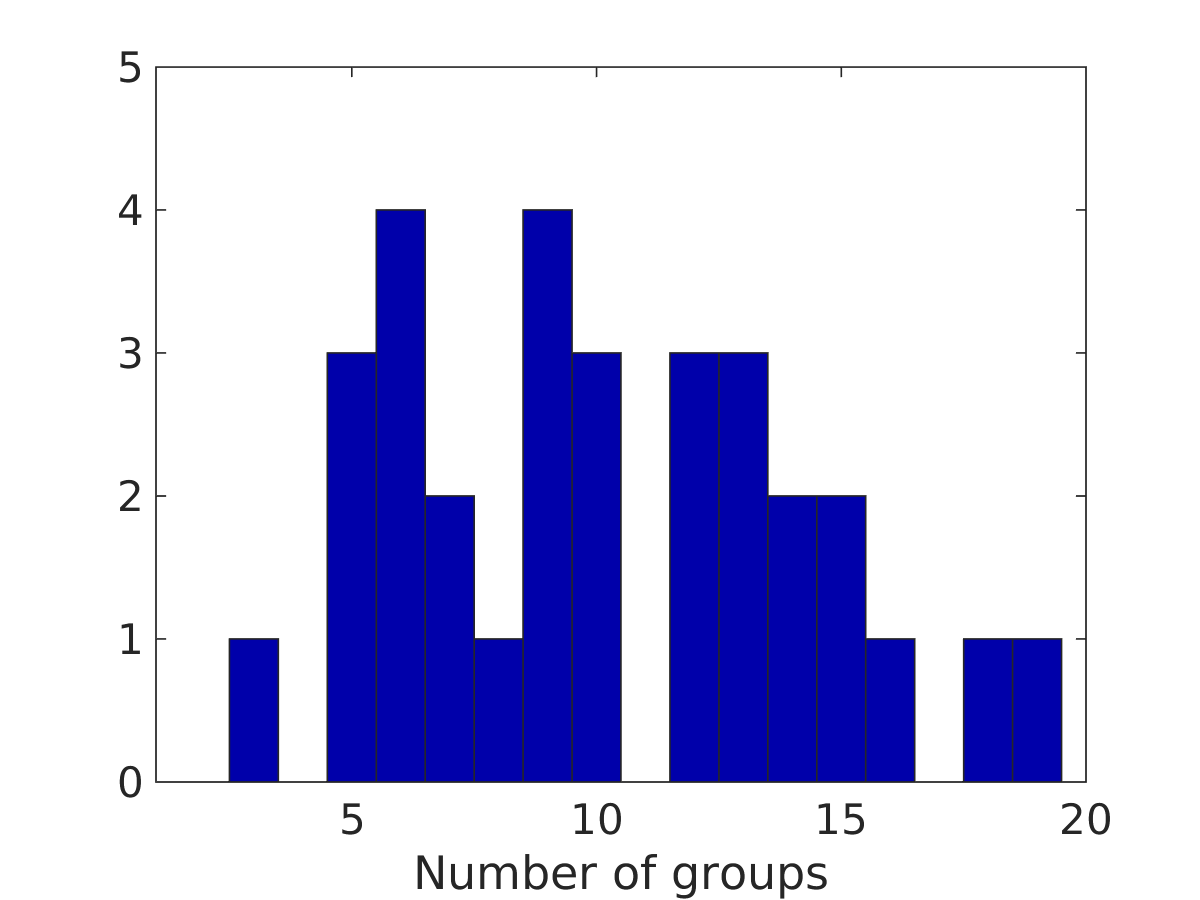
\includegraphics[width = \textwidth]{figures/nbc.png} &
  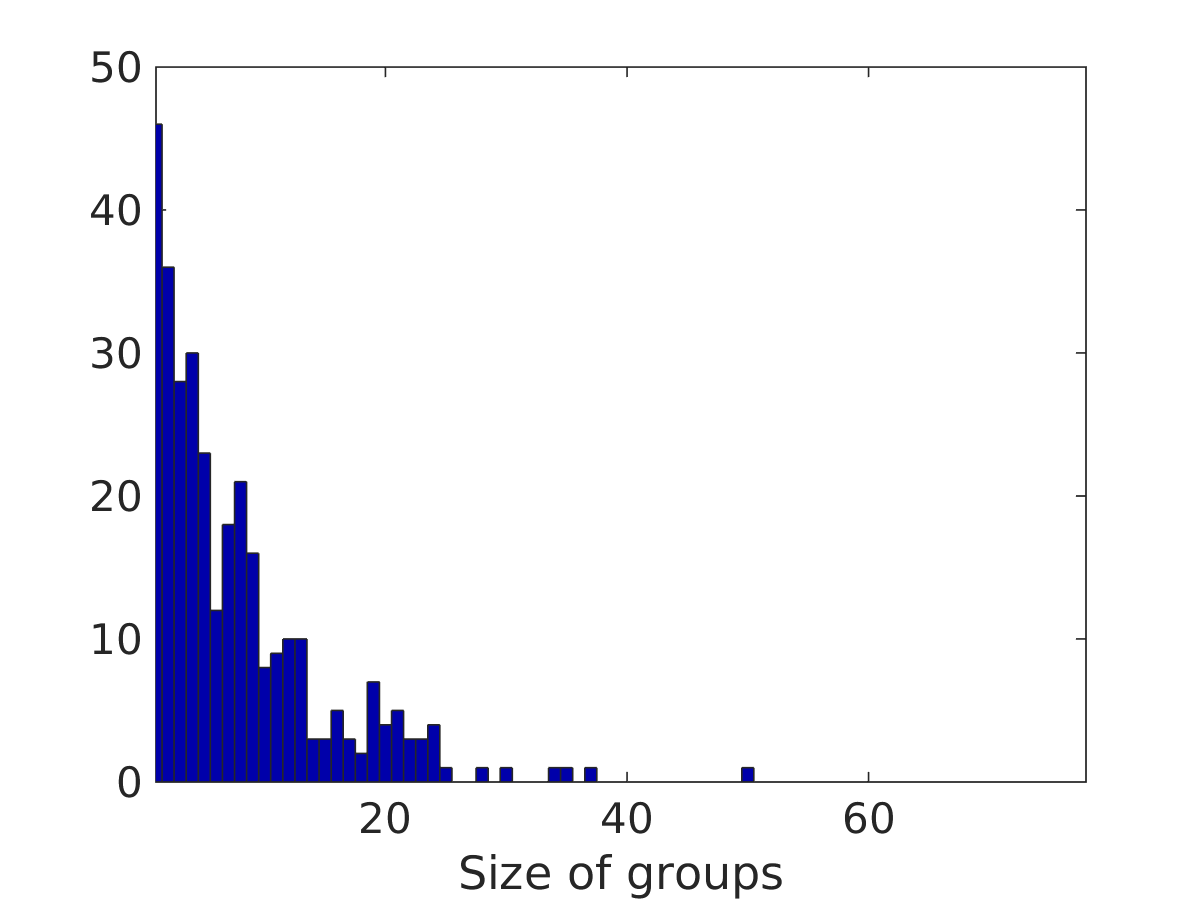
\includegraphics[width = \textwidth]{figures/sbc.png}
\end{tabular}
\caption{Histogram of the number of clusters (a) and the size of the clusters (b) defined by the $31$ subjects.}
\label{fig:xp2nbSize}
\end{figure}




%%%%%%%%%%%%%%%%%%%%%%%%%%%%%%%%%%%
%%                               %%
%% Figures                       %%
%%                               %%
%% NB: this is for captions and  %%
%% Titles. All graphics must be  %%
%% submitted separately and NOT  %%
%% included in the Tex document  %%
%%                               %%
%%%%%%%%%%%%%%%%%%%%%%%%%%%%%%%%%%%

%\section*{Figures}




%%%%%%%%%%%%%%%%%%%%%%%%%%%%%%%%%%%
%%                               %%
%% Tables                        %%
%%                               %%
%%%%%%%%%%%%%%%%%%%%%%%%%%%%%%%%%%%

% \section*{Tables}
% \begin{table}[h!]
% \caption{Sample table title. This is where the description of the table should go.}
%       \begin{tabular}{cccc}
%         \hline
%            & B1  &B2   & B3\\ \hline
%         A1 & 0.1 & 0.2 & 0.3\\
%         A2 & ... & ..  & .\\
%         A3 & ..  & .   & .\\ \hline
%       \end{tabular}
% \end{table}

%%%%%%%%%%%%%%%%%%%%%%%%%%%%%%%%%%%
%%                               %%
%% Additional Files              %%
%%                               %%
%%%%%%%%%%%%%%%%%%%%%%%%%%%%%%%%%%%

\section*{Additional Files}
  \subsection*{Additional file 1 --- Sample additional file title}
    Additional file descriptions text (including details of how to
    view the file, if it is in a non-standard format or the file extension).  This might
    refer to a multi-page table or a figure.

  \subsection*{Additional file 2 --- Sample additional file title}
    Additional file descriptions text.

\end{backmatter}

\end{document}
